%%%%%%%%%%%%%%%%%%%%%%% file typeinst.tex %%%%%%%%%%%%%%%%%%%%%%%%%
%
% This is the LaTeX source for the instructions to authors using
% the LaTeX document class 'llncs.cls' for contributions to
% the Lecture Notes in Computer Sciences series.
% http://www.springer.com/lncs       Springer Heidelberg 2006/05/04
%
% It may be used as a template for your own input - copy it
% to a new file with a new name and use it as the basis
% for your article.
%
% NB: the document class 'llncs' has its own and detailed documentation, see
% ftp://ftp.springer.de/data/pubftp/pub/tex/latex/llncs/latex2e/llncsdoc.pdf
%
%%%%%%%%%%%%%%%%%%%%%%%%%%%%%%%%%%%%%%%%%%%%%%%%%%%%%%%%%%%%%%%%%%%


\documentclass[runningheads,a4paper]{llncs}
\usepackage[utf8]{inputenc}
\usepackage{amssymb}
\setcounter{tocdepth}{3}
\usepackage{graphicx}

\usepackage{url}

\newcommand{\keywords}[1]{\par\addvspace\baselineskip
\noindent\keywordname\enspace\ignorespaces#1}

\usepackage{algorithmic}
\usepackage{algorithm}
\usepackage{mathtools,xparse}


% your email address goes here
\urldef{\mailsa}\path|your-emails@suffix| 
\newcommand{\ud}{\,\mathrm{d}}
\newcommand{\ngbf}[1]{\mathbf{#1}}
\newcommand{\gbf}[1]{\boldsymbol{#1}}
\newcommand{\E}{\mathrm{E}}
\newcommand{\Cov}{\operatorname{Cov}}
\newcommand{\diag}{\operatorname{diag}}
\newcommand{\EI}{\operatorname{EI}}
\newcommand{\PI}{\operatorname{PI}}
\renewcommand{\P}{\operatorname{P}}

\DeclarePairedDelimiter{\norm}{\lVert}{\rVert}
\newcommand{\mcite}[1]{[Fehlendes Zitat: #1]}
\newcommand{\hvs}{SMS-EMOA}
%------------------------------------------------------------------------75
\newcommand{\xx}{{\bf x}}
\newcommand{\XX}{\mathbf{X}}
\newcommand{\RBB}{\mathbb{R}}
\newcommand{\ndim}{d}
\newcommand{\ybf}{\mathbf{y}}
\newcommand{\SBB}{\mathbb{S}}
\newcommand{\shat}{\hat{s}}
\newcommand{\FCAL}{\mathcal{F}}
\newcommand{\fine}{\hspace*{\fill}$\Box$}

\graphicspath{{img/}}

%\parskip 2pt 
%\raggedbottom

\begin{document}

\mainmatter  % start of an individual contribution

% first the title is needed
\title{Applying ACO to tower defense routing}

% a short form should be given in case it is too long for the running head
\titlerunning{ACO on Tower Defense}

% the name(s) of the author(s) follow(s) next
%
% NB: Chinese authors should write their first names(s) in front of
% their surnames. This ensures that the names appear correctly in
% the running heads and the author index.
%
\author{Matthias Müller-Brockhausen \and Mark van Koningsfeld}
%
\authorrunning{Matthias Müller-Brockhausen \and Mark van Koningsfeld}
% (feature abused for this document to repeat the title also on left hand pages)

% the affiliations are given next; don't give your e-mail address
% unless you accept that it will be published
\institute{Leiden Institute of Advanced Computer Science\\
Leiden University, Niels Bohrweg 1, 2333 CA Leiden, The Netherlands}

%
% NB: a more complex sample for affiliations and the mapping to the
% corresponding authors can be found in the file "llncs.dem"
% (search for the string "\mainmatter" where a contribution starts).
% "llncs.dem" accompanies the document class "llncs.cls".
%

\toctitle{Lecture Notes in Computer Science}
\tocauthor{Authors' Instructions}
\maketitle


\begin{abstract}
We apply Ant Colony Optimization to route creeps within a Tower Defense Game. We try out different routing strategies, and play around with the rest of the parameters influencing the simulation. We then evaluate which strategy performs best under which parameters and conclude that some of the strategies are very well suited for the task.
\end{abstract}




\section{Introduction}
\label{sec:introduction}
Ant Colony Optimization is \cite[P. xy]{dorigo2006ant}

\section{Implementation}
\label{sec:implementation}
This chapter is split up into two subparts: Tech-Stack and Actual Implementation. The Tech-Stack findable in Section \ref{sec:implementationtech}, explains the libraries and techonolgies that enable our implementation. The Actual Implementation in Section \ref{sec:implementationactual} covers how we ensured a minimally working tower-defense game.

\subsection{Technical Stack}
\label{sec:implementationtech}
For our expirment to work, we require a programatically executable and influencable version of a tower defense game. There are definitely many open-source solutions out there\footnote{A search on github for "tower defense" in javascript returned 380 results.\cite{githubtowerdef}}, but for our ant colony optimization applicability we only require a very basic and simple implementation, so we decided to quickly roll out our own. How this actual Implementation looks is laid out in Section \ref{sec:implementationactual}

For the implementation we chose to create a web-tool through the usage of Javascript as a programming langauge. It provides the major advantage that, if we want to let someone else run our program to verify our conclusions, they can simply visit a link in their browser, be it mobile, desktop or gaming-console, to interact with our tool and visually see creeps deciding their ways and the pheromone-levels on the street slowly increasing\cite{curran2012future}.

We will be using typescript\cite{libstypescript} as an intermediate language to Javacsript because it supports react's JSX-Syntax per default so no need to use a transpiler like babel, and having type-suggestions etc. increases developer workflow speed as well as eases understanding of code for other team-members.

In order to make sure changes do not break any existing behavior we use the test runner called \textit{jest}\cite{libsjest}. It comes with the handy utility  \textit{matchSnapshot}\footnote{Example Usage see Section \ref{src:testgamesim}}, which allows us to match the whole current gamestate against a snapshot and immediately see unwanted changes if they occur. This \textit{matchSnapshot}-Function is also capable of capturing a snapshot of our entire UI-render, which means we are able to achieve 100\%-Line-Code-Coverage

In order to be able to easily implement the UI and add Animations merely based on the state of the game we chose to opt for \textit{react}\cite{libsreact}, with the easy \textit{velocity-react}\cite{libsreactvelocity} animation extension. With this we only have to write the position that we want for example an creep to be displayed at for the current tick, and \textit{velocity-react} remembers the previous values and makes sure that the changes in position values are then animated. This creates the illusion of the creeps walking along the path as the ticks progress\footnote{Actual Code see Section \ref{src:uiant}}. This also inherently comes with some weird animation behavior, for example when setting the tickspeed to high then the creeps position animation is merely from start to finish so it may appear to not walk on a valid street while in the backend it definitely did. Also with each change in the tick there is a slight "freeze" in the movement of the creeps.

\subsection{Actual Implementation}
\label{sec:implementationactual}

In order to Implement a tower defense game one has to identify the key-objects that play different roles in the game namely that is
\begin{itemize}
\item The walkable path with special start and target point
\item Ants walking along this path
\item Towers trying to damage these Ants
\end{itemize}
First of we store our whole map-state as well as the map-layout itself in a single class called \textit{GameField}\footnote{Source-Code in Section \ref{src:logicgame}}. The game should hold a simple 2 dimensional coordinate system, that has an x and y (width and height) constraint, so we can place our key-objects within the Field. Towers\footnote{Source-Code in Section \ref{src:logictower}} and Street\footnote{Source-Code in Section \ref{src:logicstreet}}-Parts both originate from the class \textit{Tile}\footnote{Source-Code in Section \ref{src:logictile}} which lets us position them within the coordinate system of the \textit{GameField} and makes sure they cannot overlap.
The Streets are a simple adjacency List meaning each street-part only knows its previous and next nodes and nothing else. This makes our street-network a simple network suitable for ACO. Streets also have a list of creeps that are currently on them and the current numerical pheromone level we introduced in Section \ref{sec:introduction}. This is already all the data needed for the \textit{Ant}\footnote{Source-Code in Section \ref{src:logicant}}-Class to make it's ACO-Based Routing decisions!
The Tower is also very simple it has a range, damage amount per hit and amount of hits per tick. Each Tick it will look for all streets in range and then attack as many creeps as possible. It will try to damage creeps that are the furthest and have the fewest HP first.

Bringing all this domain-logic to a visually interpretable is also pretty simple with the given data-structure. For each Tile we simply display a basic square via an HTML-\textit{div}-Element. Since we have a certain x and y-limit for our GameField mentioned earlier, we can calculate the exact width, height and position of each tile width within our window-JS-Object\cite[P. 570]{goodman2002dynamic}.

Each Game Instance also holds a variable that determines what algorithm the Ant's use to determine which node to walk to next, and how strongly pheromones are influenced and how they decay. Through that we will be able to run different kinds of experiments on different maps.

The Game itself is Tick-Based. In each tick we first spawn our new creeps. The amount of that is always variable between 0 and a configurable maximum. Aft all tower's deal all their damage. After that all alive creeps decide where they walk to next. After that has happened the general decay of pheromones is processed if enabled.

This is already all the implementation. To sum it all up: We have an isolated GameField-Class that can instantiate a whole test-setup including map, creeps and tick-progression. This GameField can either be visually rendered with results for manual verification as done in Section \ref{sec:manualver} or be run headless as in section \ref{sec:autover} to collect large amounts of data which is necessary for meaningful conclusions given that ACO behavior is stochastic.


\section{Experiments}
\label{sec:experiments}
Ant Colony Optimization is \cite[P. xy]{dorigo2006ant}

\section{Results}
\label{sec:results}
This section is divided into two subsections. First we present the results of manual experiments that we obtained by hand via the UI that we implemented in section \ref{sec:manualver}.
The second section \ref{sec:autover} contains results we obtained and evaluated automatically by running the simulations headlessly.

\subsection{Manual Verifications}
\label{sec:manualver}
This experiment was used to prove that the setup we built could find the shortest path in the three mentioned maps. For each map we tested how much time or steps it took to find an optimized path, How much creeps were created to find the path and how much of them arrived at the end point before the shortest path was found. We did not only test this with the basic ACO algorithm but also with the weighted shortest path algorithm to see if the results would be different. For every map we ran the experiment five times to see what the average result would be so that one irregular result would not influence our end result. Every time we ran the experiment until a pheromone level of 0.8 was reached in a path. 

Overall we found out that it was possible for our system to find the shortest path using the rules from the ACO algorithm. In the first map with an obvious shorter path about 30 iterations were needed to fully reinforce the optimized path. In this map the weighted shortest path algorithm had about the same results. In the second map where no obvious shortest path was present because there were twoo shortest path it took an average of 43 ticks to the point that one path was fully optimized. Here the weighted shortest path took much longer because the pheromones on both paths would keep getting increased by a little.  

In the third, more complicated maze map there started to be instances where the optimal route would not be found or would be longer than the real shortest path. This had several reasons. The first reason we found is that the decay of pheromones would already take too much of the pheromones away before the next wave would reach the path. When we took this decay away waves started going in loops because they would start reinforcing themselves. This problem was the biggest while using the weighted ACO algorithm. Because of the bigger complexity of the map there would also be a chance that a wrong path would already get reinforced before all routes were tried. The time also took longer with an average of 79 ticks before an optimum was found. 

After we added towers to the maps we noticed that the results were very similar with amounts of creeps it took to reach an optimum, depending on how the towers were placed. In the basic algorithm no pheromones were added when creeps did not reach the end of the path. This meant that creeps would find routes around the towers when the creeps would not be able to get through and even when they did there would be way more using the longer routes. When it was less obvious which path was the best because we placed multiple towers it would take longer to create an optimum.

\subsection{Automatic Evaluation Results}
\label{sec:autover}
For the automatic evaluation we tried varying settings and ran them across all maps. Because the amount of different parameters and the hence large amount of graphs to interpret we will here only mention and display the settings that we deemed relevant information. To be statistically relevant every experiment setting is run 50 times and we then take the mean value of that for the graph. We also always include Towers in the maps.

Regarding the settings when we talk about normal settings, then these are the settings we found to work best using the manual mode. This consist of a spawn-amount of 14, a decay-threshold of -0.007 and a pheromone-increase threshold of 0.01.

First of we will start out by excluding the continuous vapor in the future Figures because as Figure \ref{fig:mirrorvaptick} clearly shows, the runtime is much larger than for all other three behaviors for the mirrored map. This behavior was visible across all maps and settings, another example that stresses the uselessness of the continuous vapor is the runtime graph portrayed in Figure \ref{fig:shortlongvaptick} for the short and long map, the very basic map that all of them should be able to easily master.

\begin{figure}[H]
  \centering
  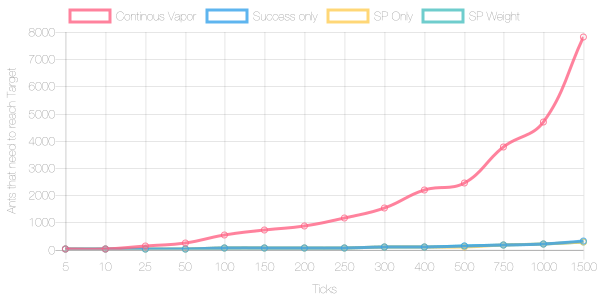
\includegraphics[width=1\linewidth]{images/normalmirroredwithtower-ticks-line}
  \caption{Comparing required Tick-Amount on the y-Axis to the target amount of creeps to reach the target on the x-Axis for the mirrored map with normal settings.}
  \label{fig:mirrorvaptick}
\end{figure}

\begin{figure}[H]
  \centering
  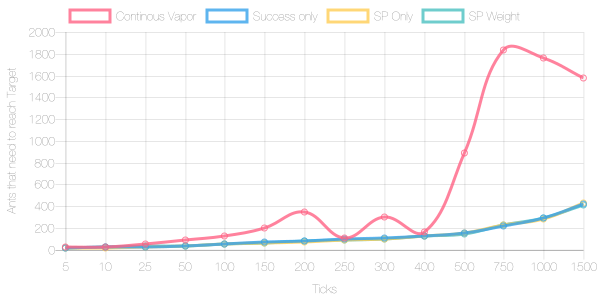
\includegraphics[width=1\linewidth]{images/normalshortandlongwithtowers-ticks-line}
  \caption{Comparing required Tick-Amount on the y-Axis to the target amount of creeps to reach the target on the x-Axis for the short and long map with normal settings}
  \label{fig:shortlongvaptick}
\end{figure}

With the automatic evaluation we also further prove, that deducing pheromones upon death is rather counter-productive than helpful as visible in Figure \ref{fig:deathsubshitty}. But it does make sense given that any street-part an ant crossed on it's way to death will be deduced in pheromone. That means even a correct path like in the short and long map the longer one can lead to pheromone deduction and hence make the path unattractive again and future ants more likely to walk the even more dangerous path with more deaths.
Also for the weighted shortest path leaving death-substraction out even slightly improves the result. As for the non continuous vapor behavior, not only does substraction not matter as much, but also all three perform quite similar.


\begin{figure}[H]
  \centering
  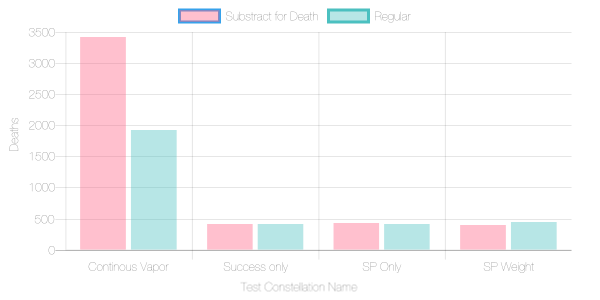
\includegraphics[width=1\linewidth]{images/normalshortandlongwithtowers-deaths}
  \caption{Comparing deaths for the different creep behaviors with and without substracting pheromones upon death on the short and long map with normal settings}
  \label{fig:deathsubshitty}
\end{figure}

The following graph, depicted in Figure \ref{fig:threesame} which doesn't include the continuous vapor any more shows, shows that the remaining three behaviors perform similar not only regarding death amount but also regarding their runtime.

\begin{figure}[H]
  \centering
  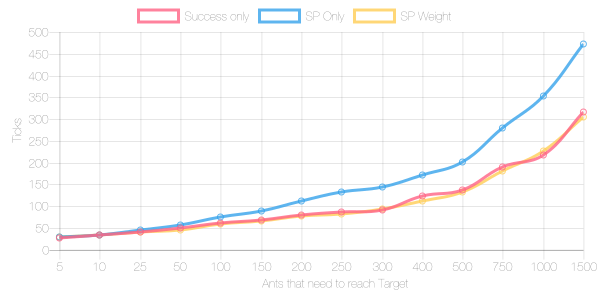
\includegraphics[width=1\linewidth]{images/normalsquaremaze-ticks-line}
  \caption{Comparing required Tick-Amount on the y-Axis to the target amount of creeps to reach the target on the x-Axis for the maze map with normal settings}
  \label{fig:threesame}
\end{figure}

Because of that similarity we ran another experiment only using the shortest weighted path algorithm, but with a few differing settings. The result of that is accessible through Figure \ref{fig:diffsettings} which portrays the amount of Ticks and Figure \ref{fig:diffsettingsdeath} which displays the amount of deaths.

As we can see using a high spawn rate with no or low decay will result in much more deaths than usual. Manually reconstructing this scenario with the UI explains why that is: With a high spawn rate many ants come through every way regardless of the tower strength. Hence bad ways can be reinforced and made attractive even though they are not.
Another possible conclusion is that using a low spawn rate in combination with no or low decay will increase runtime, which is logical given that the target is the amount of ants that need to reach the target and less spawned ants mean less ants per tick are able to arrive at the target. 

\begin{figure}[H]
  \centering
  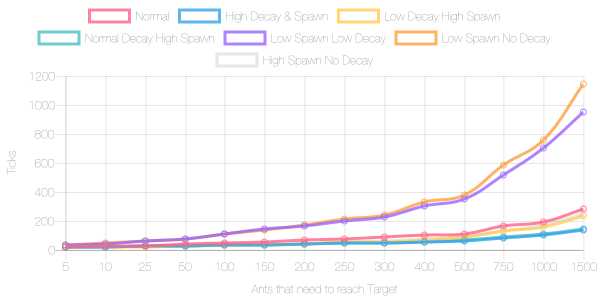
\includegraphics[width=1\linewidth]{images/mirroredwithtower-ticks-line}
  \caption{Comparing required Tick-Amount on the y-Axis to the target amount of creeps to reach the target on the x-Axis for the mirrored map with normal settings}
  \label{fig:diffsettings}
\end{figure}

\begin{figure}[H]
  \centering
  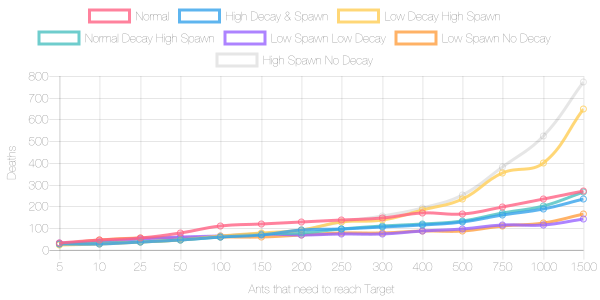
\includegraphics[width=1\linewidth]{images/mirroredwithtower-deaths-line}
  \caption{Comparing amount of deaths on the y-Axis to the target amount of creeps to reach the target on the x-Axis for the mirrored map with normal settings}
  \label{fig:diffsettingsdeath}
\end{figure}

We have also already shown that the spawn-amount only has a logical impact on the tick amount and 14 is a good number given the damage of the towers. Now we also want to prove that the pheromone increase and decrease-level we declared as \textit{normal} are optimal
For that Figure \ref{fig:diffsettings2} compares the amount of ticks and Figure \ref{fig:diffsetting2sdeath} the amount of deaths for different pheromone-settings with the spawn amount 14 on the mirrored map.

As we can see the best value is in both instances achieved by the completely normal settings. It also shows that a low increase or also decay can negatively influence runtime. Also using a low pheromone increase can cause more deaths.

\begin{figure}[H]
  \centering
  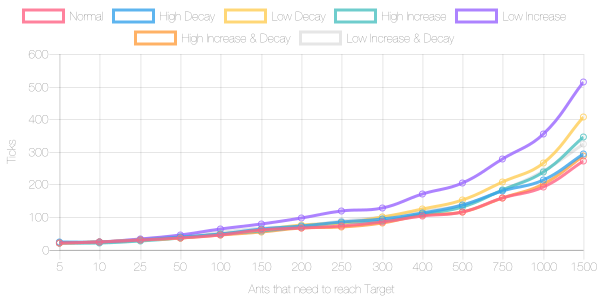
\includegraphics[width=1\linewidth]{images/mirrorednormalpheromticks}
  \caption{Comparing required Tick-Amount o n the y-Axis to the target amount of creeps to reach the target on the x-Axis for the mirrored map with varying settings}
  \label{fig:diffsettings2}
\end{figure}

\begin{figure}[H]
  \centering
  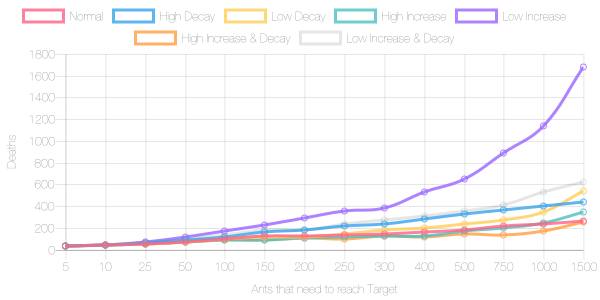
\includegraphics[width=1\linewidth]{images/mirroredwittowerdeaths}
  \caption{Comparing amount of deaths on the y-Axis to the target amount of creeps to reach the target on the x-Axis for the mirrored map with normal settings}
  \label{fig:diffsetting2sdeath}
\end{figure}

\section{Conclusion}
\label{sec:conclusion}
We have presented the basics of a tower defense game and of ant colony optimization. With these basics we were able to show that the algorithms can be usefully applied to tower defense games.
For this tower defense implementation we have built a Web-UI that can be run in any browser. It enables the re-verification of our manual experiments (section \ref{sec:manualver}) as well as custom new experiments on the pre-made maps.
To better evaluate the different routing algorithms (section \ref{sec:behaviour}), we run many experiments headlessly with many run throughs for statistical relevance (section \ref{sec:autover}).

Concluding from both these experiments we can say that Ant Colony Optimization can produce useful results in a Tower Defense Game. Shortest Path with or without weight and on success only are viable options to route through a maze, but the weighted one will produce the least deaths. We also showed that we have found optimal parameters for the experiments by showing that different settings yield worse results (section \ref{sec:autover}).

There are still many more map constellations, ant behaviour modifications, differing towers and more to try out as pointed out in the future work section \ref{sec:futurework}, but we successfully achieved a working ant colony optimization routing for tower defense games.

\section{Appendix}
\label{sec:appendix}
\section{Source Code for GameField-Class}
\label{src:logicgame}
UI-Ant-Code

\section{Source Code for Tile-Class}
\label{src:logictile}
UI-Ant-Code

\section{Source Code for Street-Class}
\label{src:logicstreet}
UI-Ant-Code

\section{Source Code for Tower-Class}
\label{src:logictower}
UI-Ant-Code

\section{Source Code for Ant-Class}
\label{src:logicant}
UI-Ant-Code

\section{Source Code for Ant-Displayment}
\label{src:uiant}
UI-Ant-Code

\section{Source Code for Game-Simulation Test}
\label{src:testgamesim}
Test-Code Game-Simulation



%
% The following two commands are all you need in the
% initial runs of your .tex file to
% produce the bibliography for the citations in your paper.
%\bibliographystyle{abbrv}
%\bibliography{main}  % sigproc.bib is the name of the Bibliography in this case
% You must have a proper ".bib" file
%  and remember to run:
% latex bibtex latex latex
% to resolve all references
%
% ACM needs 'a single self-contained file'!
%
%APPENDICES are optional
%\balancecolumns
\bibliographystyle{abbrv}
\bibliography{report} 

\end{document}
